\chapter{Measurements from IMU}\label{app:IMUMeasurementsAppendix}
\textbf{Name: Group 630}\\
\textbf{Date: 15/04 - 2016}

\subsubsection{Purpose}
Analyse the data coming from the IMU, specifically the accelerometer and and the gyroscope measurements and calculating the angle \si{\theta_F} from those measurements.


\subsubsection{Setup}
The setup for this test is the Cubli setup on a table and the code made by the previous group working with the Cubli. From it the Linear state feedback controller is selected \fxnote{put old code in CD appendix}
%\begin{figure}[H]                                   
%	\centering                                        
%	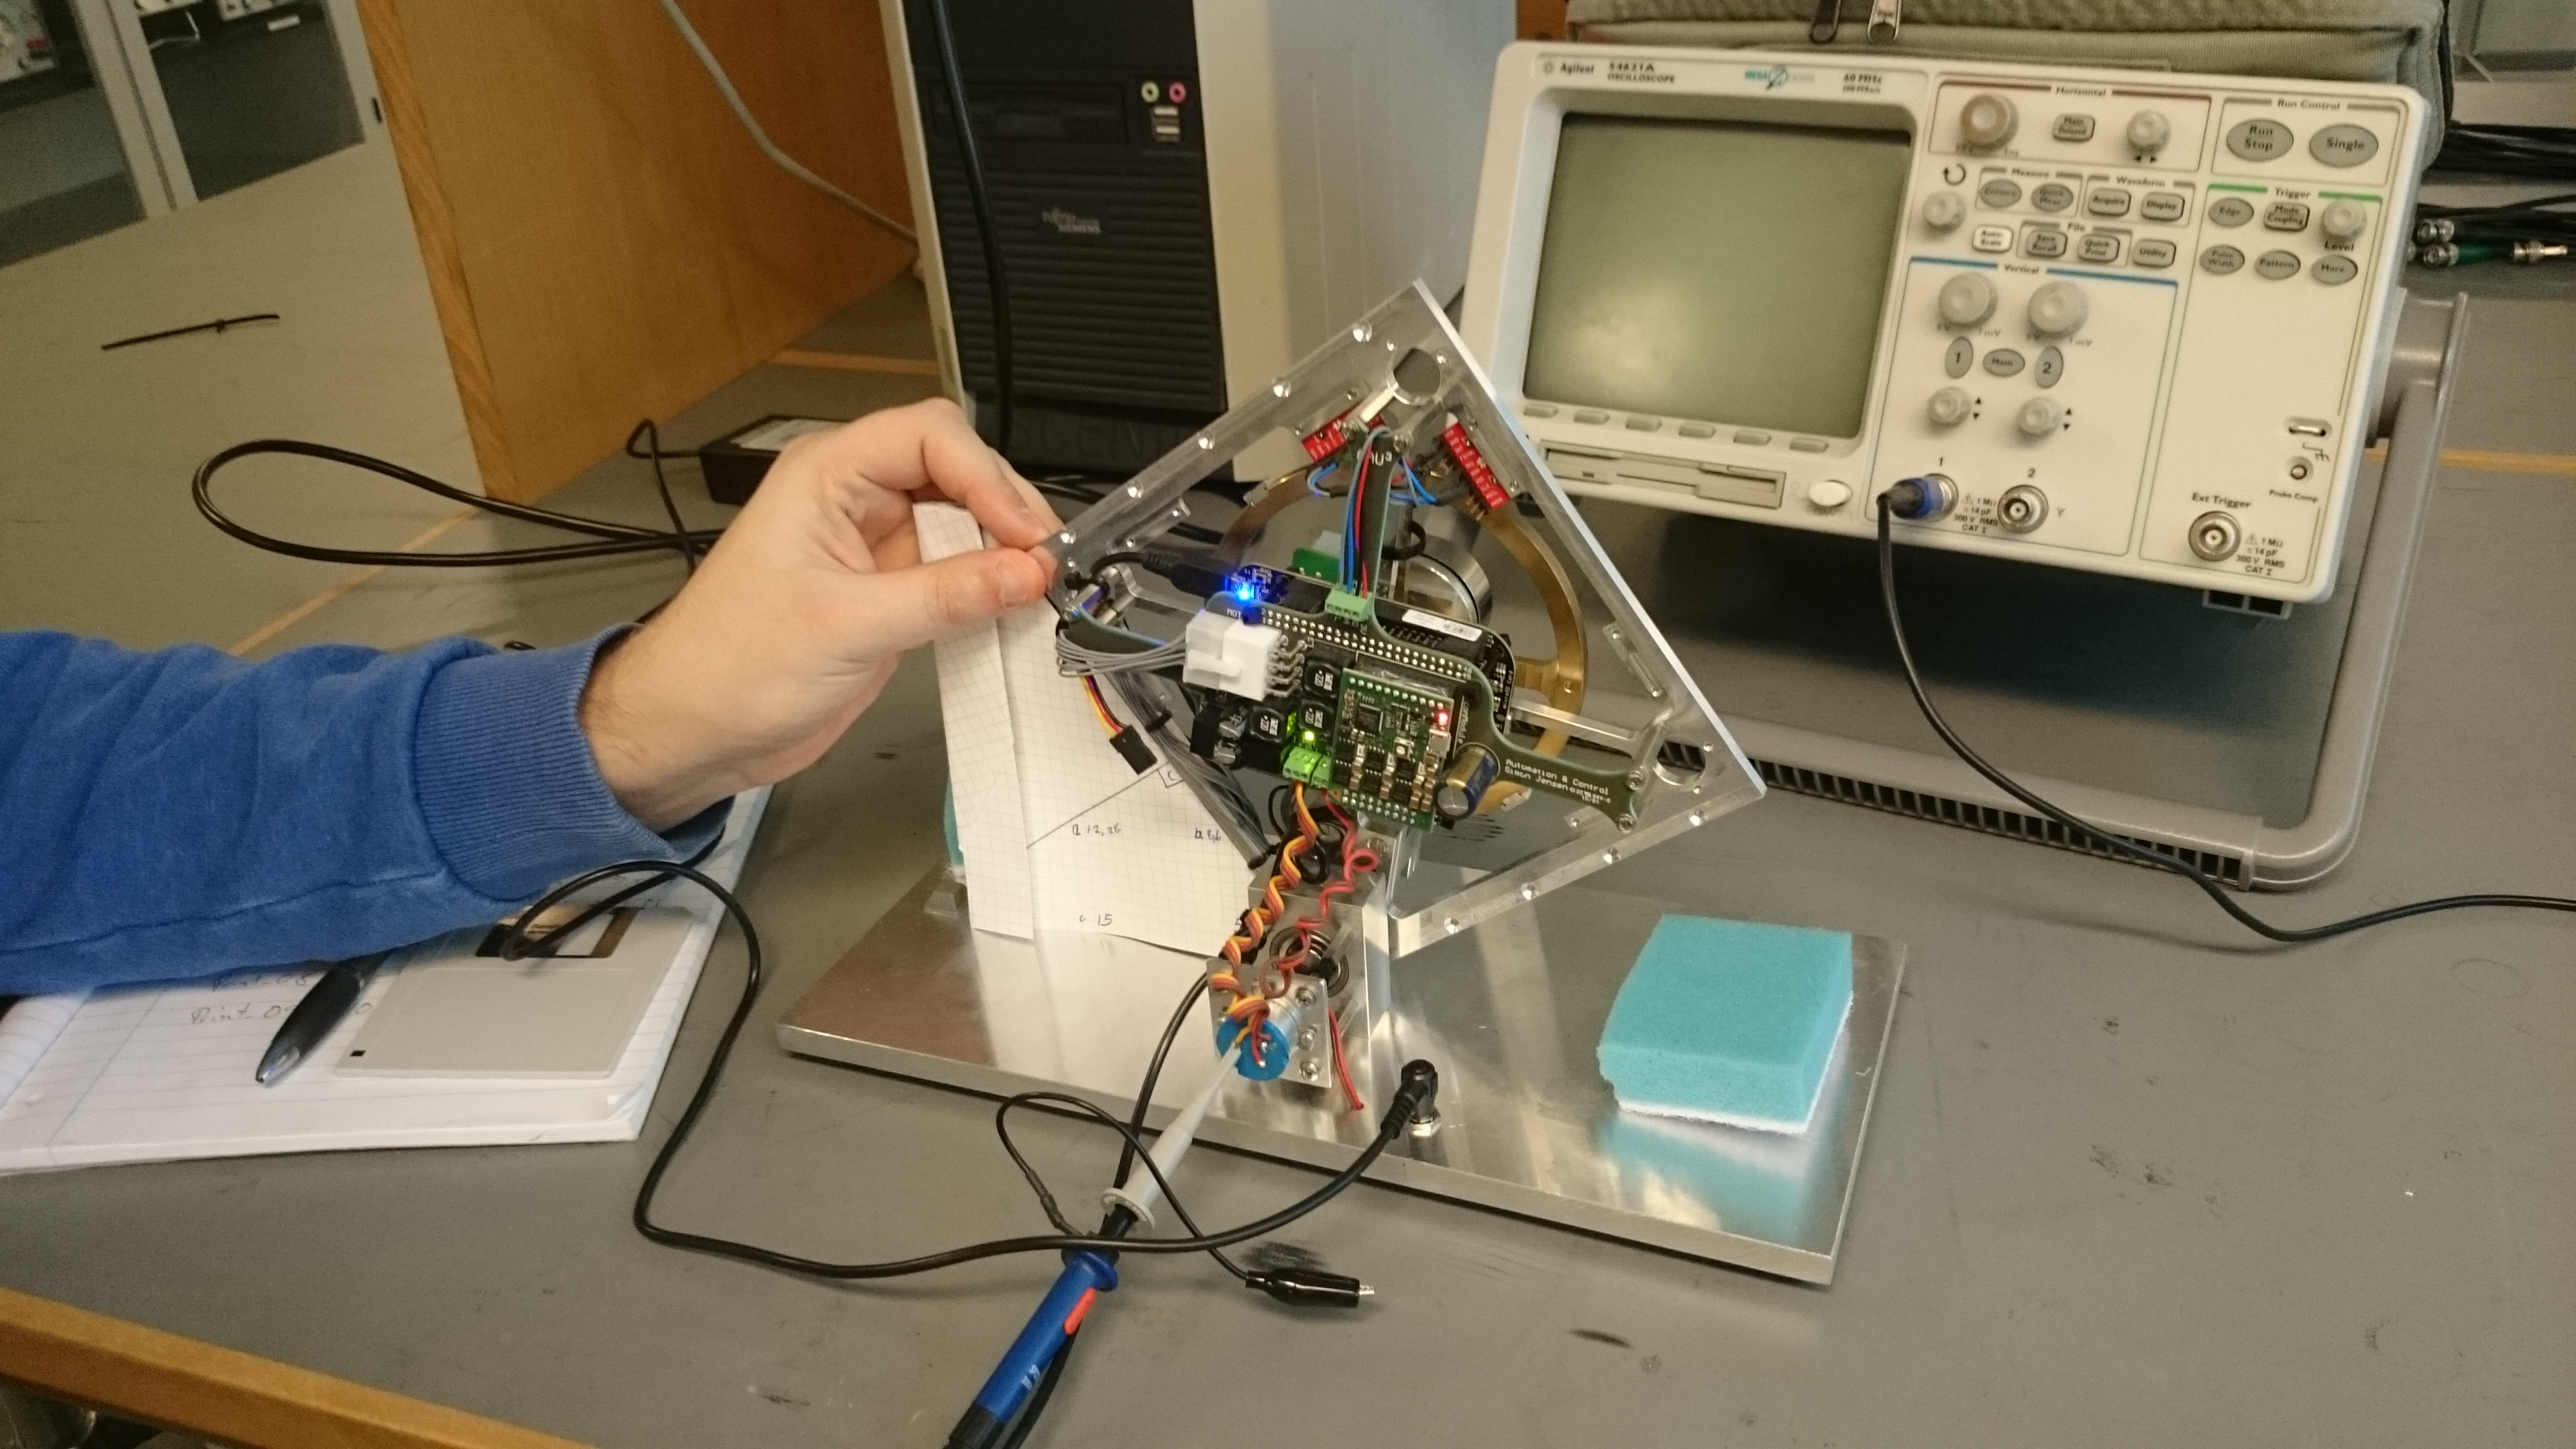
\includegraphics[scale=0.08]{figures/stepResponseSetup}
%	\caption{Picture of the data measurement test}
%	\label{dataMeasurementIMUPicture} 
%\end{figure}              

\subsubsection{List of Equipment}
\begin{table}[H]
	\begin{tabular}{|l|l|p{4.3cm}|}
		\hline%------------------------------------------------------------------------------------
		\textbf{Instrument}                        &  \textbf{AAU-no.}  &  \textbf{Type}       \\
		\hline%------------------------------------------------------------------------------------
		Cubli setup                              &               &  		  \\
		\hline%------------------------------------------------------------------------------------
		Dedicated Power Supply of Cubli \small{(24 V - 3 A)} &               &  XP Power, AEB70US24 \\
		\hline%------------------------------------------------------------------------------------
		PC with the code from simon                &              &            \\
		\hline%------------------------------------------------------------------------------------
	\end{tabular}
\end{table}
\subsubsection{Procedure}
\begin{enumerate}
	%\item Turn on the power supply
	\item Assign a new name to the data file measurements are saved to in the code
	\item Upload the code with Simons Linear state feedback controller activated
	\item Start the program and let the cubli balance for a few seconds
	\item Poke the Cubli a few times so there is some random variations in the angle
	\item Take the measurements and plot them in Matlab
	%\item Plot the result of the simulations in the same figure and compare them
\end{enumerate}


\subsubsection{Results}
The measured data is partially converted through the code. Accelerometer and gyro values are given in rad/s. \fxnote{might need changing if we have to redo the conversion, B}
Data from the accelerometer is converted into an angle with arctan and the gyro data is integrated because the gyroscope is measuring the angular velocity in the direction of the frames rotation. This is done to see how close the potentiometer the angle the data comes.
The data is available as a .csv file on the CD\fxnote{Make sure this is put into the CD folder for copying}

To find the angle from the accelerometer data is done the following equation:
\begin{flalign}
	&\si{\theta_{F}=\arctan(\frac{y_1}{x_1})}&
	\label{eq:accelToAngle}
\end{flalign}

\begin{figure}[H] 
	\centering 
	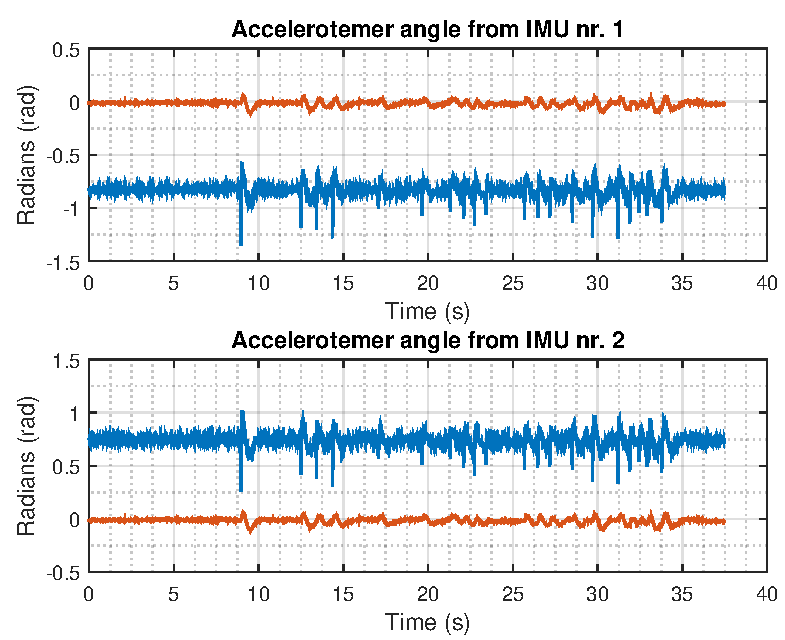
\includegraphics[scale=0.8]{figures/acc1}
	\caption{Test 1, accelerometer angle (blue) compared to the angle from the potentiometer (orange)}
	\label{data1acc}
\end{figure}
\begin{figure}[H] 
	\centering 
	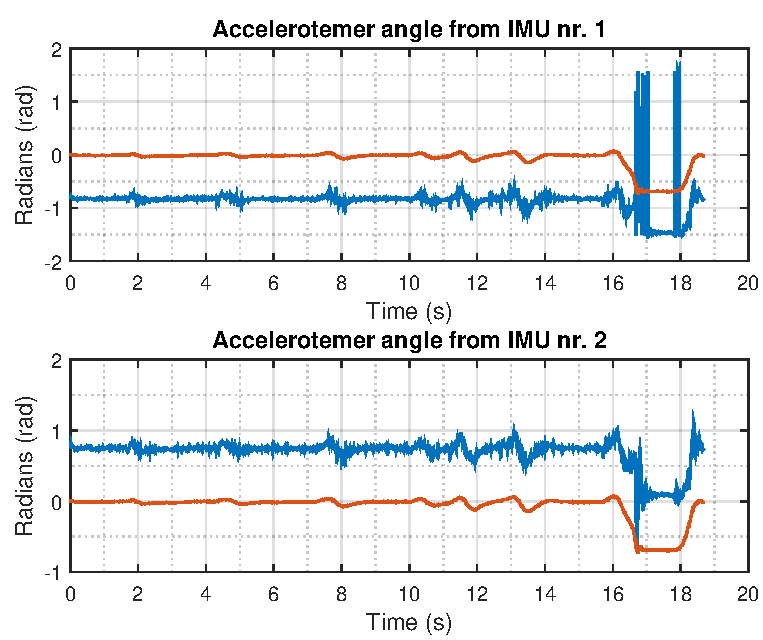
\includegraphics[scale=0.8]{figures/acc2}
	\caption{Test 2, accelerometer angle (blue) compared to the angle from the potentiometer (orange)}
	\label{data2acc}
\end{figure}
\begin{figure}[H] 
	\centering 
	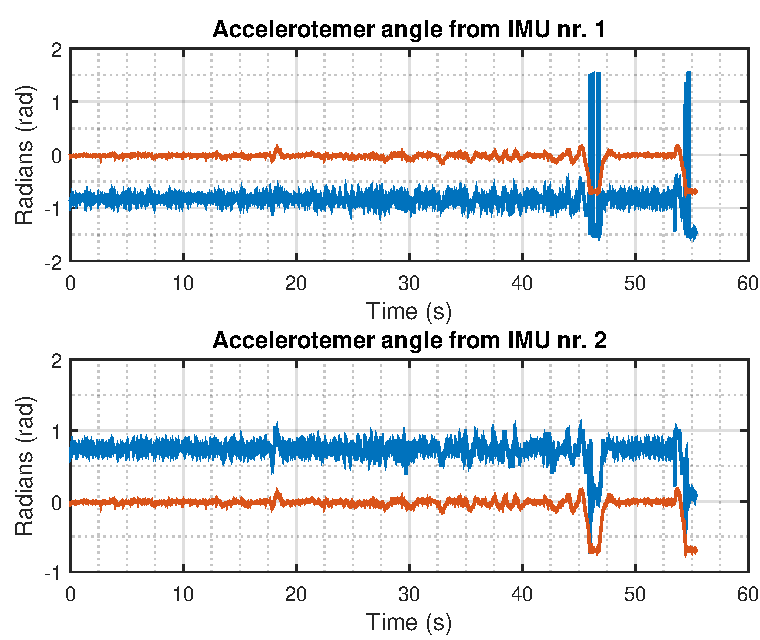
\includegraphics[scale=0.8]{figures/acc3}
	\caption{Test 3, accelerometer angle (blue) compared to the angle from the potentiometer (orange)}
	\label{data3acc}
\end{figure}
\begin{figure}[H] 
	\centering 
	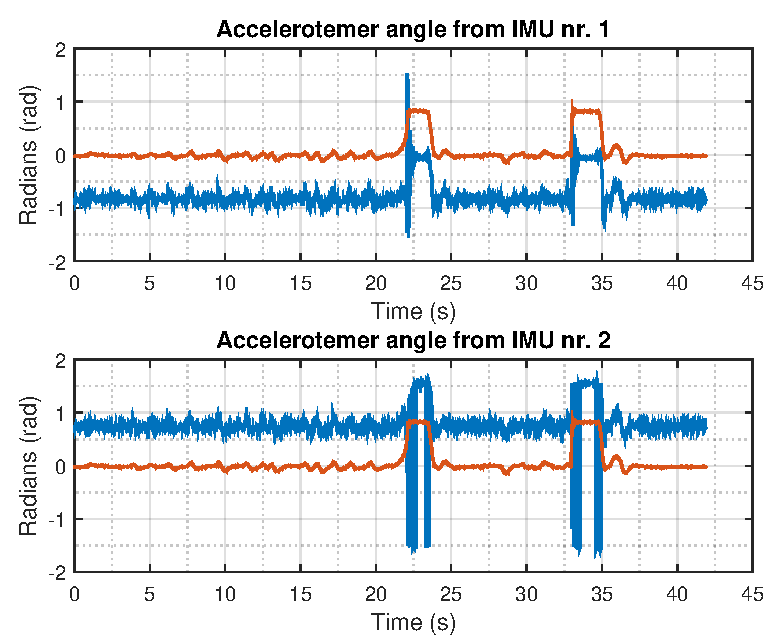
\includegraphics[scale=0.8]{figures/acc4}
	\caption{Test 4, accelerometer angle (blue) compared to the angle from the potentiometer (orange)}
	\label{data4acc}
\end{figure}

The gyroscopes angular velocity measurement is integrated.
The integration is done the same way it would be done in the code on the BeagleBone.
\begin{flalign}
	&\si{\theta_{F}[n]=\theta_{F}[n-1]+\omega[n] \cdot \Delta T}&
	\label{eq:gyroToAngle}
\end{flalign}

\si{\Delta T} being the samplingfrequency of the controller.
\begin{figure}[H] 
	\centering 
	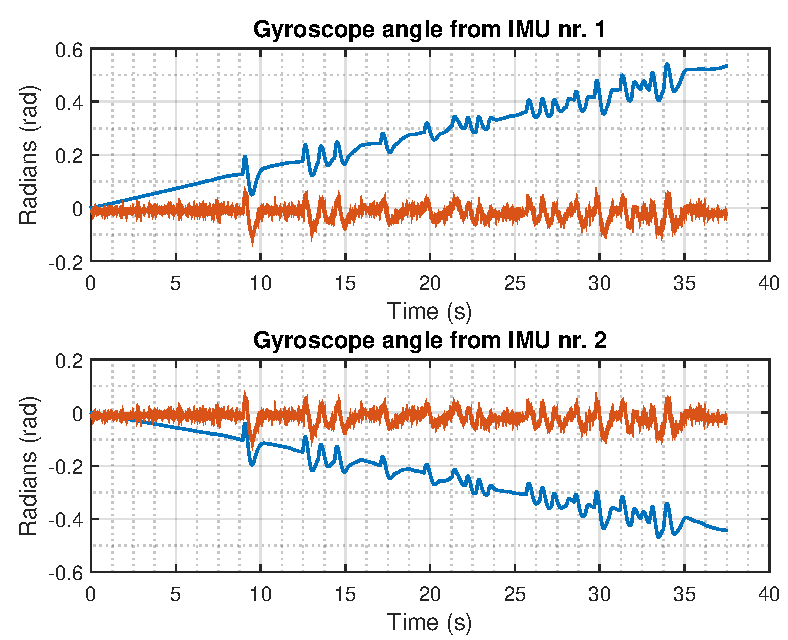
\includegraphics[scale=0.8]{figures/gyro1}
	\caption{Test 1, gyroscope angle (blue) compared to the angle from the potentiometer (orange)}
	\label{data1gyro}
\end{figure}
\begin{figure}[H] 
	\centering 
	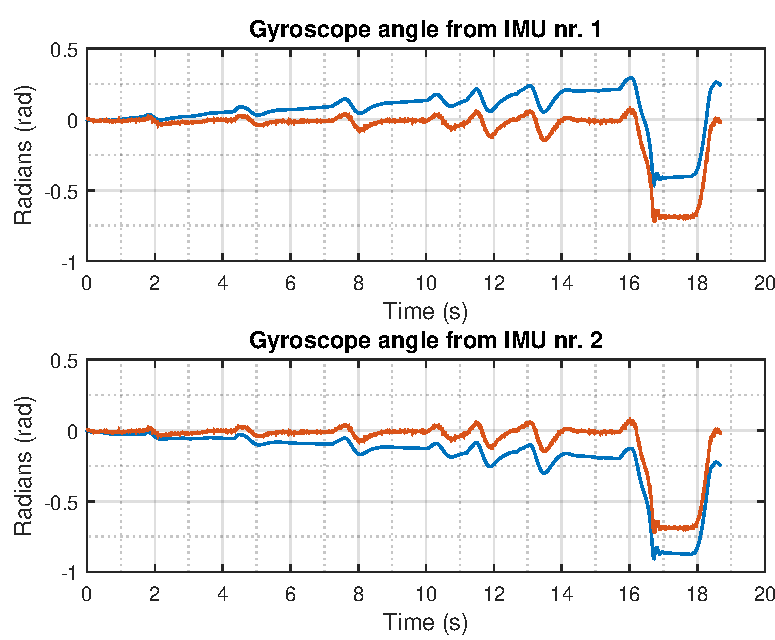
\includegraphics[scale=0.8]{figures/gyro2}
	\caption{Test 2, gyroscope angle (blue) compared to the angle from the potentiometer (orange)}
	\label{data2gyro}
\end{figure}
\begin{figure}[H] 
	\centering 
	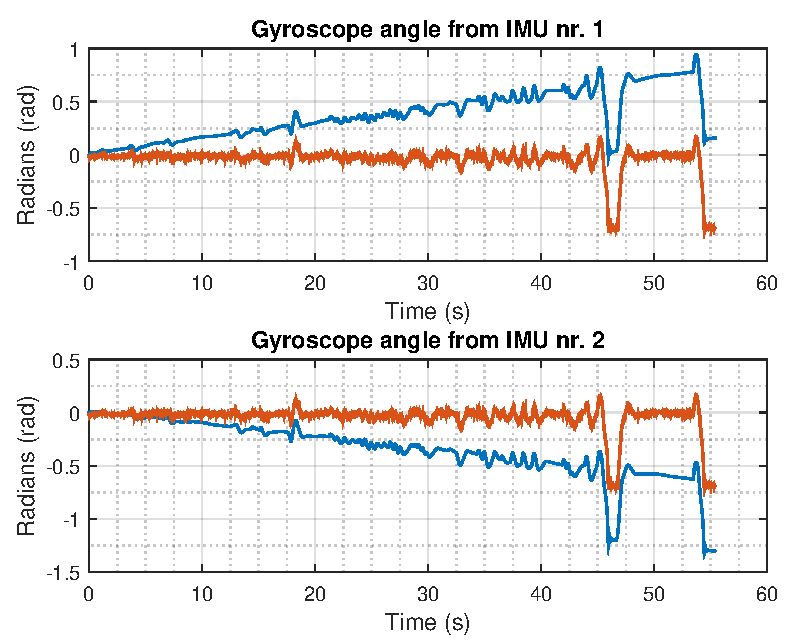
\includegraphics[scale=0.8]{figures/gyro3}
	\caption{Test 3, gyroscope angle (blue) compared to the angle from the potentiometer (orange)}
	\label{data3gyro}
\end{figure}
\begin{figure}[H] 
	\centering 
	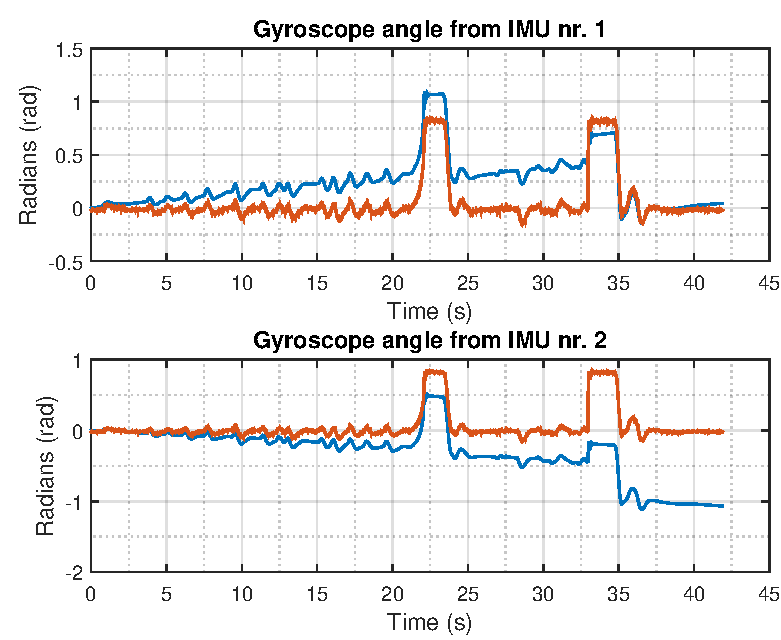
\includegraphics[scale=0.8]{figures/gyro4}
	\caption{Test 4, gyroscope angle (blue) compared to the angle from the potentiometer (orange)}
	\label{data4gyro}
\end{figure}

\subsubsection{Note}
There is a constant offset in the accelerometer data. Also it can be seen that there is some noise in the measurements, especially when there are rapid movements.

It can be observed that the gyroscope data has an increasing offset in the data. This offset comes from the integration of the angular velocity, that the gyroscope measures.